\documentclass{beamer}

\usetheme{Frankfurt}
\setbeamertemplate{navigation symbols}{}

\title{A dynamic audio routing system\\based on the RSSI of a Bluetooth device}
\author{Davide Pesavento, Martina Astegno}
\date{\today}

\begin{document}

\begin{frame}[plain]
\titlepage
	\begin{center}
		Universit\`{a} degli Studi di Padova \\
		Corso di Laurea Magistrale in Informatica
	\end{center}
\end{frame} 
 
\begin{frame}
	\frametitle{Outline}
	\tableofcontents 
\end{frame}

%_____________________%

\section{Introduction}

	\begin{frame}
		\frametitle{Project's aim}
		The \textbf{GOAL} of our application can be divided into two different parts: 
		\pause
		\begin{itemize}
		\item to use Bluetooth technology to locate a person among a set of possible rooms;
		\pause
		\item to playback sound among these rooms dinamically swiching it, from one speaker to another, according to person's movements. 
		\end{itemize}    
	\end{frame}
	
	\begin{frame}
		\frametitle{Tecnologies adopted}
		We adopted two principal tecnologies:
		\pause
		\begin{itemize}
		\item \textbf{Bluetooth} technology for short range wireless communications. We adopted BlueZ as Bluetooth stack implementation.\\ \textbf{HCI} status parameter $\rightarrow$ RSSI value to detect the nearest adapter to the person. 
		\pause
		\item \textbf{Pulseaudio}, a sound server that acts as proxy for sound applications. It redirects audio streams according to person's movements or allows simoultaneos playbacks by more speakers. 
		
		\end{itemize}
	\end{frame}
	
	\begin{frame}
		\frametitle{Hardware requirements}
		To run the application there are some basic hardware requirements:
		\pause
		\begin{itemize}
		\item \textbf{Smartphone}, to identify the room in which the person is.
		\item \textbf{Central server}, to host the main control application.
		\end{itemize}
		\pause
		And for each rooms:
		\begin{itemize}
		\item a \textbf{speaker} that lets out sound when selected for playback;
		\item a \textbf{Bluetooth adapter} that detects the RSSI value and sends it to the server.
		\end{itemize}
		
		 
		
	\end{frame}
	
%_____________________%

\section{Main project modules}

	\begin{frame}
		\frametitle{Bluetooth module}
		\textbf{Probe:} a simple application implemented for each BT adapter. It can interface with BlueZ throught DBus.\\
		\vspace{0.5cm}
		\texttt{ProbeManager}
		\begin{itemize}
		\item monitors device localization;
		\item stores information about every \texttt{ProbeInterface}
		\end{itemize}
		\texttt{ProbeInterface}
		\begin{itemize}
		\item starts/stops discovery;
		\item updates RSSI values when a change occurs.
		\end{itemize}
		%The main HCI commands used in our implementation are:
		%\begin{itemize}
		%\item Link Control Commands, to search for other devices in range and to establish connection to other devices;
		%\item Status Parameters Commands, to extract detailed information from the remote device. This includes the link quality and
          %the RSSI value.
		%\end{itemize}
		%The choice of the speaker that has to playback sound is based on the RSSI value provided by Status Parameters commands.
	
	\end{frame}
	
	\begin{frame}
		\frametitle{Pulseaudio module}
		The Pulseaudio basic concepts: \textbf{sink} and \textbf{sink input}\\
		\vspace{0.5cm}
		\texttt{PAController} $ \rightarrow $ the class implemented to manage and control Pulseaudio operations.
		\begin{itemize}
		\item \texttt{PAController::MoveOperation} - it redirects the sound to one or more different sinks.
		\item \texttt{PAController::LoadModuleOperation} - it performs the loading of PA modules
			\begin{itemize}
			\item \texttt{module-tunnel-sink} (tunnel connection with central server)
			\item \texttt{module-combine} (simultaneous playback)
			\end{itemize}
		\end{itemize}
	
	\end{frame}
	
%_____________________%

\section{Operating system}
	\begin{frame}
		\frametitle{Runtime behavior***TOFIX***}
		\mbox{
		\begin{minipage}[c]{5cm}
		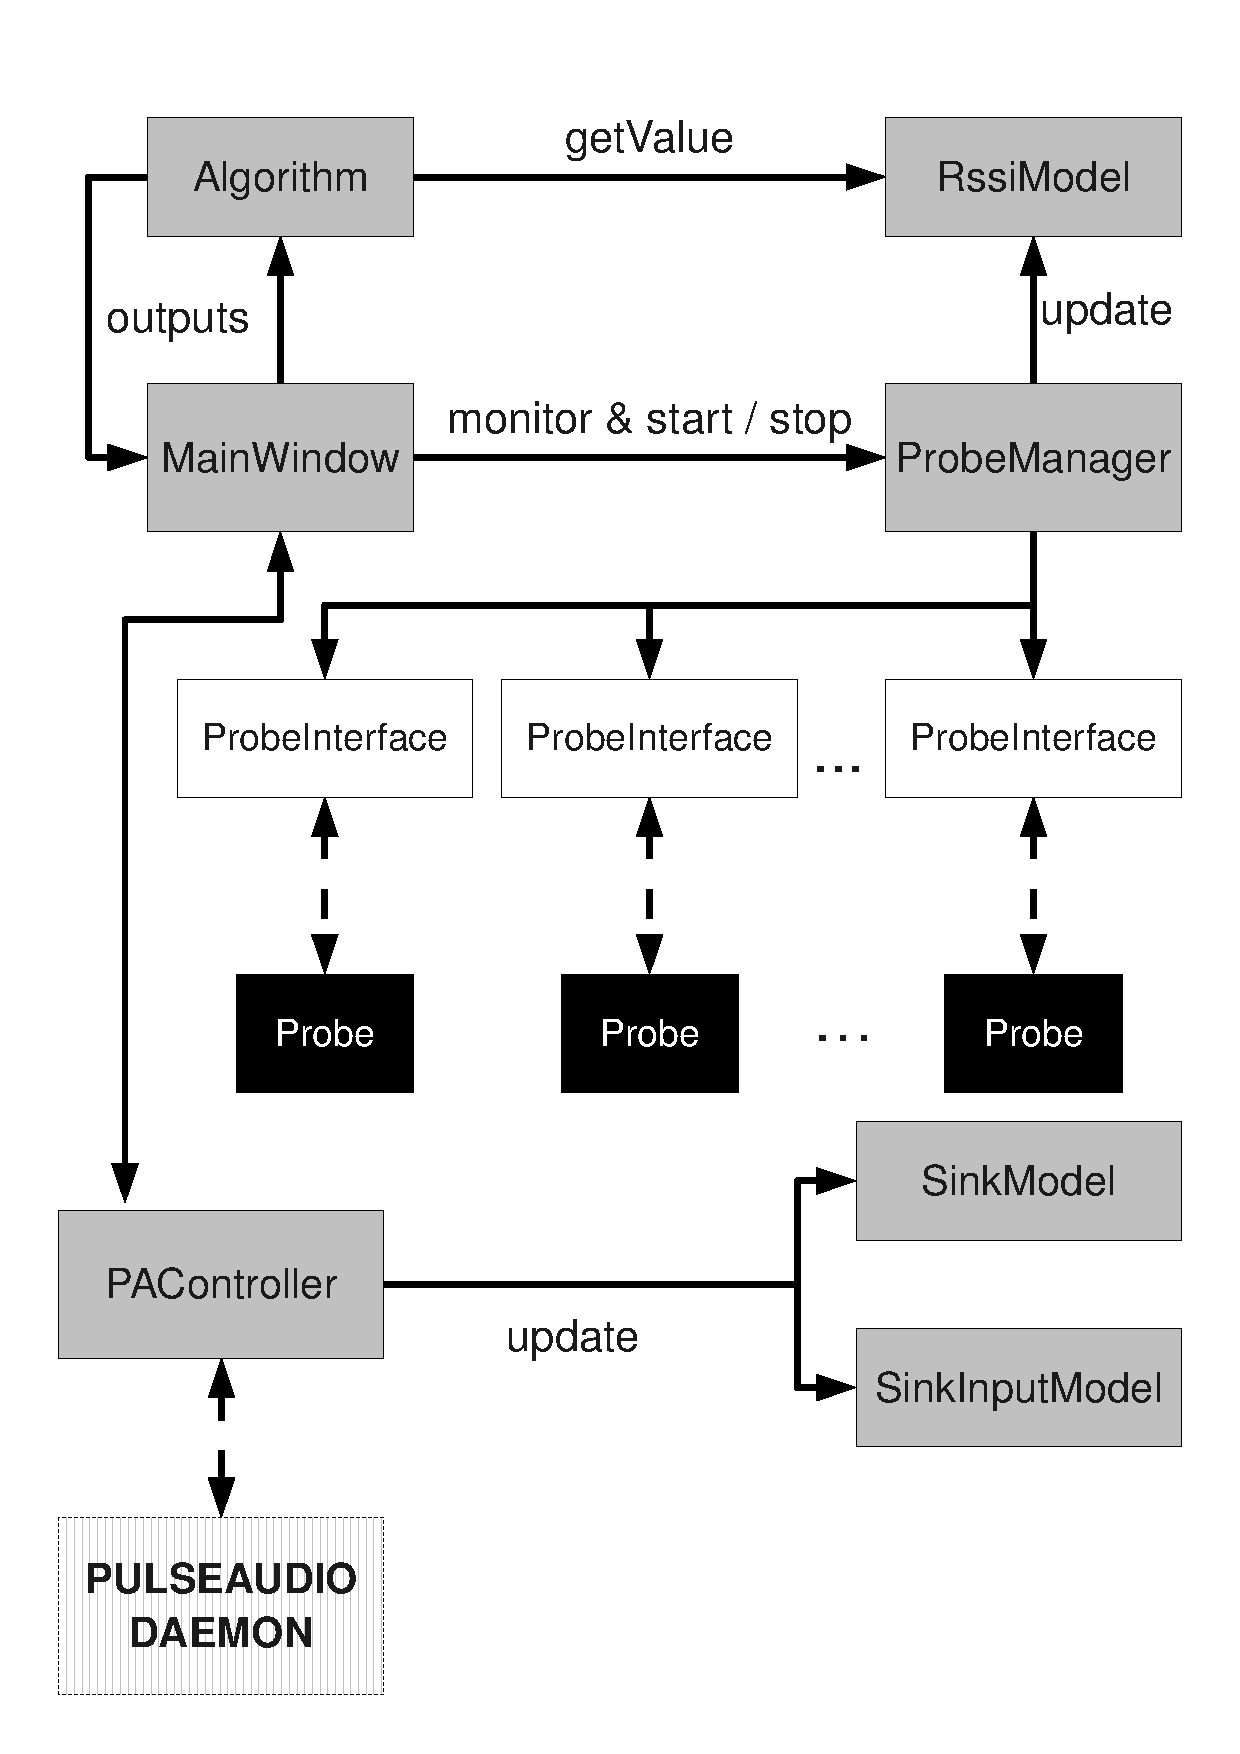
\includegraphics[scale = 0.25]{architettura.pdf}
		\end{minipage}
		\quad	
		\begin{minipage}[c]{5cm}
		\begin{enumerate}
		\item Periodically \textbf{Probes} obtain RSSI value (INQUIRY)
		\pause
		\item If difference between new and old values higher than threshold t $\rightarrow$ update \texttt{RssiModel}
		\pause
		\item Algorithm runs $\rightarrow$ output
		\pause
		\item If output differs from current room $\rightarrow$ send request to \texttt{PAController}
		\pause
		\item \texttt{PAController} updates sinks according to algorithm output
		\end{enumerate}
		\end{minipage}		
		}
	\end{frame}
	
	\begin{frame}
		\frametitle{Testing interface***YES/NO??***}
	\end{frame}
	
%______________________%

\section{Future work and possible extensions}

	
	\begin{frame}
		\frametitle{Future extensions}
		\begin{itemize}
		\item Real world testing: ....
		\pause
		\item Multiple devices managing: it could be interesting to consider a context with more than one device to locate. In this case it's necessary to evaluate how different devices could interact.
		\pause
		\item Control's user addition: mobile application that allows to the user to control the audiostream (adjust volume, stop/pause, next/previous, \ldots)
		\end{itemize}
	\end{frame}
	
%______________________%

\section{Conclusions}
	\begin{frame}
		\frametitle{Final considerations***TODO***}
	\end{frame}


\end{document}
